%--------------------------------------------------------------------
% NE 155 (intro to numerical simulation of radiation transport)
% Spring 2014

% formatting
\documentclass[12pt]{article}
\usepackage[top=1in, bottom=1in, left=1in, right=1in]{geometry}

\usepackage{setspace}
\onehalfspacing

\setlength{\parindent}{0mm} \setlength{\parskip}{1em}


% packages
\usepackage{amssymb}
%% The amsthm package provides extended theorem environments
\usepackage{amsthm}
\usepackage{epsfig}
\usepackage{times}
\renewcommand{\ttdefault}{cmtt}
\usepackage{amsmath}
\usepackage{graphicx} % for graphics files

% Draw figures yourself
\usepackage{tikz} 

% The float package HAS to load before hyperref
\usepackage{float} % for psuedocode formatting
\usepackage{xspace}

% from Denovo methods manual
\usepackage{mathrsfs}
\usepackage[mathcal]{euscript}
\usepackage{color}
\usepackage{array}

\usepackage[pdftex]{hyperref}

\newcommand{\nth}{n\ensuremath{^{\text{th}}} }
\newcommand{\ve}[1]{\ensuremath{\mathbf{#1}}}
\newcommand{\macro}{\ensuremath{\Sigma}}
\newcommand{\vOmega}{\ensuremath{\hat{\Omega}}}

\newcommand{\cc}[1]{\ensuremath{\overline{#1}}}
\newcommand{\ccm}[1]{\ensuremath{\overline{\mathbf{#1}}}}


%--------------------------------------------------------------------
%--------------------------------------------------------------------
\begin{document}
\begin{center}
{\bf NE 155, Classes 21-23, S14 \\
Finite Difference Methods for the DE \\ March 12-17, 2014}
\end{center}

\setlength{\unitlength}{1in}
\begin{picture}(6,.1) 
\put(0,0) {\line(1,0){6.25}}         
\end{picture}

%--------------------------------------------------------------------
\section{Finite-Difference Method}
\underline{Problem} Consider the following second order ODE:
\[f''(x) = p(x)f'(x) + q(x)f(x) + r(x)\]
%
defined on a segment $[a,b]$ with $f(a) = \alpha$ and $f(b) = \beta$ (a boundary value problem).  

Now, let's spatially discretize the equation:
%
\begin{center}
\begin{tikzpicture}
\draw (-.25,0)--(1.25,0);
\draw[dotted] (1.25,0)--(2.75,0);
\draw (2.75,0)--(5.25,0);
\draw[dotted] (5.25,0)--(6.75,0);
\draw (6.75,0)--(8.25,0);
%\draw (4,0)--(5.25,0);
\draw (0,-.25)--(0,.25);
\draw (1,-.25)--(1,.25);
%\draw (2,-.25)--(2,.25);
\draw (3,-.25)--(3,.25);
\draw (4,-.25)--(4,.25);
\draw (5,-.25)--(5,.25);
\draw (7,-.25)--(7,.25);
\draw (8,-.25)--(8,.25);
\node[below] at (0,-.25) {$x_0 = a$};
\node[below] at (1,-.25) {$x_1$};
\node[below] at (3,-.25) {$x_{i-1}$};
\node[below] at (4,-.25) {$x_i$};
\node[below] at (5,-.25) {$x_{i+1}$};
\node[below] at (7,-.25) {$x_{n-1}$};
\node[below] at (8,-.25) {$x_n = b$};
\node[above] at (0.5, 0.5) {$h$};
\node[above] at (3.5, 0.5) {$h$};
\end{tikzpicture}
\end{center}
%
where $x_0 = a$, $x_n = b$, and $h$ is the mesh spacing. There are $n+1$ points and $n$ mesh cells.

We can use \textbf{central difference} to approximate the derivatives on this grid. Let's use the $O(h^2)$ versions:
%
\begin{align}
f'(x_i) &= \frac{f(x_i + h) - f(x_i - h)}{2h} - \frac{h^2}{6} f'''(\mu) \nonumber \\
%
f''(x_i) &= \frac{f(x_i + h) - 2f(x_i) + f(x_i - h)}{h^2} + \frac{h^2}{12}f^{(4)}(\mu) \nonumber
\end{align}
%
We will also define $p_i = p(x_i)$, $q_i = q(x_i)$, $r_i = r(x_i)$.

Substituting into the original equation, we get:
\begin{align}
\frac{f_{i+1} - 2f_i + f_{i-1}}{h^2} &= p_i \frac{f_{i+1} - f_{i-1}}{2h} + q_i f_i + r_i \qquad i = 1, 2, \dots, n-1 \nonumber \\
%
\bigl(\frac{-h}{2}p_i - 1\bigr) f_{i-1} &+ \bigl(2 + h^2q_i\bigr)f_i + \bigl(\frac{h}{2}p_i - 1\bigr) f_{i+1} = -h^2 r_i \qquad i = 1, 2, \dots, n-1 \nonumber
\end{align}

We only have $n-1$ equations, but because the boundaries are fixed that is all we need. This is clear when we look at the $i=1$ and $i=n-1$ cases:
\begin{align}
&\bigl(2 + h^2q_1\bigr)f_1 + \bigl(\frac{h}{2}p_1 - 1\bigr) f_{2} = -h^2 r_1 + \underbrace{\bigl(\frac{h}{2}p_1 + 1\bigr) \underbrace{\alpha}_{f_0}}_{bc_L} \nonumber \\
 %
&\bigl(\frac{-h}{2}p_{n-1} - 1\bigr) f_{n-2} + \bigl(2 + h^2q_{n-1}\bigr)f_{n-1} = -h^2 r_{n-1} + \underbrace{\bigl(\frac{-h}{2}p_{n-1} + 1\bigr) \underbrace{\beta}_{f_n}}_{bc_R} \nonumber
\end{align}

Thus, we can write this as a matrix equation:
\begin{equation}
\begin{pmatrix}
\bigl(2 + h^2q_1\bigr) & \bigl(\frac{h}{2}p_1 - 1\bigr) & & \hdots & 0 \\
%
\bigl(\frac{-h}{2}p_2 - 1\bigr) & \bigl(2 + h^2q_2\bigr) & \bigl(\frac{h}{2}p_2 - 1\bigr) & &  \\
\vdots & \ddots & \ddots & \ddots & \vdots \\
& & \bigl(\frac{-h}{2}p_{n-2} - 1\bigr) & \bigl(2 + h^2q_{n-2}\bigr)  & \bigl(\frac{h}{2}p_{n-2} - 1\bigr) \\
0 & \hdots & & \bigl(\frac{-h}{2}p_{n-1} - 1\bigr) & \bigl(2 + h^2q_{n-1}\bigr) \\
\end{pmatrix}
%
\begin{pmatrix}
f_1 \\ f_2 \\ \vdots \\ f_{n-2} \\ f_{n-1} \\
\end{pmatrix}
= 
\begin{pmatrix}
-h^2 r_1 + bc_L \\ -h^2 r_2 \\ \vdots \\ -h^2 r_{n-1} \\ -h^2 r_{n-1} + bc_R\\ 
\end{pmatrix}\nonumber
\end{equation}


Note: the numerical solution to the PDE is an approximation to the exact solution that is obtained using a discrete representation of the PDE at the grid points $x_i$ in the discrete spatial mesh. Let us denote this numerical solution as $F$ such that 
$$F_j \approx f(x_j)$$ 

Thus, the numerical solution is a collection of finite values
$$F = [F_1, F_2, \dots, F_{n-1}]$$
and we have boundary values $F_0$ and $F_n$.


%---------------------------------------------
\subsection{DE}
What does this look like if we apply it to the steady state 1-D diffusion equation?
\[-D\frac{d^2 \phi(x)}{dx^2} + \Sigma_a \phi(x) = S\]
\[\frac{d^2 \phi}{dx^2} - \frac{1}{L^2}\phi(x) = \frac{-S}{D}\]
and let $\phi(a) = \phi(b) = 0$ (vacuum bcs). Then we get
\begin{align}
\frac{\phi_{i+1} - 2\phi_i + \phi_{i-1}}{h^2} - \frac{1}{L^2}\phi_i &= \frac{-S_{0,i}}{D} \qquad i = 1, 2, \dots, n-1 \nonumber \\
%
-\phi_{i-1} &+ \bigl(2 + \frac{h^2}{L^2}\bigr)\phi_i - \phi_{i+1} = h^2 \frac{S_{0,i}}{D} \qquad i = 1, 2, \dots, n-1 \nonumber
\end{align}

One problem with this formulation is that we only have values at the cell edges: \underline{edge centered}. This really only works well when we have homogeneous media. Why might that be? If we have \textit{material discontinuities} it's going to be difficult to enforce flux continuity between cells. Note: $L$ and $D$ are not functions of space; we wouldn't know which cell's values to assign when using edge-centered values. 

What could we do instead? \underline{cell-centered}, which leads us to our next topic.


%-----------------------------------------------------
%-----------------------------------------------------
\section{Finite Volume Method}
Rather than pointwise approximations on a grid, FVM approximates an average integral value on a reference volume.

%
\begin{center}
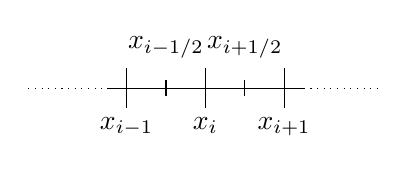
\begin{tikzpicture}
\draw[dotted] (1.75,0)--(2.75,0);
\draw (2.75,0)--(5.25,0);
\draw[dotted] (5.25,0)--(6.25,0);
\draw (3,-.25)--(3,.25);
\draw (3.5,-.1)--(3.5,.1);
\draw (4,-.25)--(4,.25);
\draw (4.5,-.1)--(4.5,.1);
\draw (5,-.25)--(5,.25);
\node[below] at (3,-.25) {$x_{i-1}$};
\node[below] at (4,-.25) {$x_i$};
\node[below] at (5,-.25) {$x_{i+1}$};
\node[above] at (3.5, 0.25) {$x_{i-1/2}$};
\node[above] at (4.5, 0.25) {$x_{i+1/2}$};
\end{tikzpicture}
\end{center}

Consider the elliptic equation $f''(x) = r(x)$ on a control volume $V_i = [x_{i-1/2}, x_{i+1/2}]$, then
\[\int_{x_{i-1/2}}^{x_{i+1/2}} f''(x)dx = \int_{x_{i-1/2}}^{x_{i+1/2}} r(x) dx\]
%
We can evaluate the lhs analytically and the rhs using some integration rule. For simplicity, let's use the midpoint rule:
%
\[f'(x_{i+1/2}) - f'(x_{i-1/2}) = (x_{i+1/2} - x_{i+1/2})r_i\]
%
We can now use differencing schemes to represent the derivatives on the left. Define $h = x_{i+1/2} - x_{i-1/2}$
\[\frac{f_{i+1} - 2f_i + f_{i-1}}{h} = hr_i\]

This
\begin{itemize}
\item applies to the integral form of conservation laws (like the DE).
\item handles discontinuities in solution (because we're using cell-integrated values)
\item works well for heterogeneous systems because each cell can be a different material
\item there exists a theory for convergence, accuracy, and stability
\end{itemize}


%---------------------------------------------
\subsection{DE} 
What does this look like if we apply it to the steady state 1-D diffusion equation?
\[-\frac{d}{dx}D(x)\frac{d \phi(x)}{dx} + \Sigma_a(x) \phi(x) = S(x)\]
%
\begin{figure}[h!]
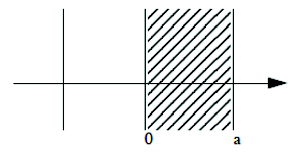
\includegraphics[height=1in]{FVM-fig}
\end{figure}
%
Let's also assume we have an equilibrium (reflecting) condition at the centerline ($x_0 = 0$) and vacuum on the right ($x_n = a$):
\begin{align}
\frac{d}{dx}\phi(x) \big|_{x=0} &= 0 \qquad \text{zero net current} \nonumber\\
\phi(\tilde{a}) &= 0 \qquad \tilde{a} = a + 2D \nonumber
\end{align}

We again have a spatial mesh, and material discontinuities will coincide with cell edges, $x_i$. Thus, we assume the cross section and diffusion coefficient are constant in each cell and the unknown fluxes and known sources are defined at the cell edges:
\begin{align}
D(x) &= D_i\;, \qquad x_{i-1} \leq x \leq x_i \nonumber \\
\Sigma_a(x) &= \Sigma_{a,i}\;, \qquad x_{i-1} \leq x \leq x_i \nonumber \\
h_i &\equiv x_{i} - x_{i-1} \nonumber \\
\phi(x_i) &= \phi_i \nonumber \\
S(x_i) &= S_i \nonumber 
\end{align}
%
\begin{figure}[h!]
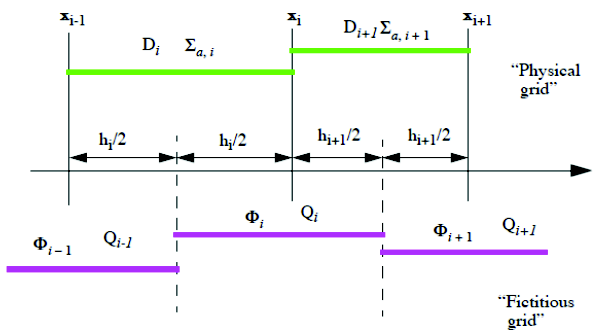
\includegraphics[height=2.5in]{FVM-DE}
\end{figure}

We further assume that the fluxes and sources are constant over the interval centered around $x_i$:
%
\begin{align}
\phi(x) &= \phi_i \qquad \text{for } \bigl(x_i - \frac{h_i}{2}\bigr) \leq x \leq \bigl(x_i + \frac{h_{i+1}}{2}\bigr) \nonumber \\
S(x) &= S_i \qquad \text{for } \bigl(x_i - \frac{h_i}{2}\bigr) \leq x \leq \bigl(x_i + \frac{h_{i+1}}{2}\bigr) \nonumber 
\end{align}

Now, we integrate the differential equation over each cell, $\bigl(x_i - \frac{h_i}{2}\bigr) \leq x \leq \bigl(x_i + \frac{h_{i+1}}{2}\bigr)$:
%
\[\int_{(x_i - \frac{h_i}{2})}^{(x_i + \frac{h_{i+1}}{2})} \biggl(  -\frac{d}{dx}D(x)\frac{d \phi(x)}{dx}\biggr) dx + \int_{(x_i - \frac{h_i}{2})}^{(x_i + \frac{h_{i+1}}{2})} \Sigma_a(x) \phi(x) dx = \int_{(x_i - \frac{h_i}{2})}^{(x_i + \frac{h_{i+1}}{2})} S(x) dx\]

Term by term:
\begin{align}
\int_{(x_i - \frac{h_i}{2})}^{(x_i + \frac{h_{i+1}}{2})} S(x) dx &\approx S_i \bigl(\frac{h_i + h_{i+1}}{2}\bigr) \qquad \text{defined at cell edge} \nonumber \\
&\nonumber\\
\int_{(x_i - \frac{h_i}{2})}^{(x_i + \frac{h_{i+1}}{2})} \Sigma_a(x) \phi(x) dx &= 
\int_{(x_i - \frac{h_i}{2})}^{(x_i)} \Sigma_a(x) \phi(x) dx + \int_{(x_i)}^{(x_i + \frac{h_{i+1}}{2})} \Sigma_a(x) \phi(x) dx \nonumber\\&=
\biggl(\frac{\Sigma_{a,i}h_i + \Sigma_{a,i+1}h_{i+1}}{2} \biggr)\phi_i\nonumber \qquad \text{defined at cell center}\\
&\nonumber\\
 \int_{(x_i - \frac{h_i}{2})}^{(x_i + \frac{h_{i+1}}{2})} \biggl(  -\frac{d}{dx}D(x)\frac{d \phi(x)}{dx}\biggr) dx &=
-\biggl[D(x)\frac{d \phi(x)}{dx} \biggr]_{(x_i - \frac{h_i}{2})}^{(x_i + \frac{h_{i+1}}{2})} \qquad \text{defined at cell edge}\nonumber \\
%
-D(x)\frac{d \phi(x)}{dx}\big|_{(x_i + \frac{h_{i+1}}{2})} &\cong -D_{i+1}\biggl(\frac{\phi_{i+1} - \phi_i}{h_{i+1}}\biggr) \nonumber \\
%
-D(x)\frac{d \phi(x)}{dx}\big|_{(x_i - \frac{h_i}{2})} &\cong -D_{i}\biggl(\frac{\phi_{i} - \phi_{i-1}}{h_{i}}\biggr) \nonumber
\end{align}

Collecting all of the terms:
%
\begin{equation}
-D_{i+1}\biggl(\frac{\phi_{i+1} - \phi_i}{h_{i+1}}\biggr) + D_{i}\biggl(\frac{\phi_{i} - \phi_{i-1}}{h_{i}}\biggr) + \biggl(\frac{\Sigma_{a,i}h_i + \Sigma_{a,i+1}h_{i+1}}{2} \biggr)\phi_i =   S_i \bigl(\frac{h_i + h_{i+1}}{2}\bigr) \nonumber
\end{equation}

We can express this in matrix form, but we'll use some abbreviations to make it more compact:
\begin{align}
h_{ii} &= \frac{h_i + h_{i+1}}{2} \nonumber \\
%
\Sigma_{a,ii} &= \frac{\Sigma_{a,i}h_i + \Sigma_{a,i+1}h_{i+1}}{h_i + h_{i+1}} \nonumber \\
\end{align}
Divide through by $h_{ii}$, then
%
\[a_{i,i-1} \phi_{i-1} + a_{i,i}\phi_i + a_{i, i+1} \phi_{i+1} = S_i \qquad \text{for } i = 1, 2, \dots, n-1\]
%
where
%
\begin{align}
a_{i,i-1} &= \frac{-D_i}{h_i h_{ii}} \nonumber \\
a_{i,i} &= \frac{D_i}{h_i h_{ii}} + \frac{D_{i+1}}{h_{i+1} h_{ii}} +\Sigma_{a,ii} \nonumber \\
a_{i,i+1} &= \frac{-D_{i+1}}{h_{i+1} h_{ii}} \nonumber
\end{align}

Now we have a set of $n-1$ linear algebraic equations with $n+1$ unknowns. Next up: boundary conditions.


%-------------------------------------------------------
\subsection{Boundary Conditions}

If we assume $x_n = \tilde{a}$, then the \textbf{vacuum condition} becomes
\[\phi_n = 0\]
and the last equation for $i=n-1$ becomes
\[a_{n-1,n-2} \phi_{n-2} + a_{n-1,n-1}\phi_{n-1} + a_{n-1, n} \times 0 = S_{n-1}\]

Next we'll worry about the \textbf{reflecting} or zero current condition. The first step is to integrate over $[0, h_{1}/2]$.
%
\begin{figure}[h!]
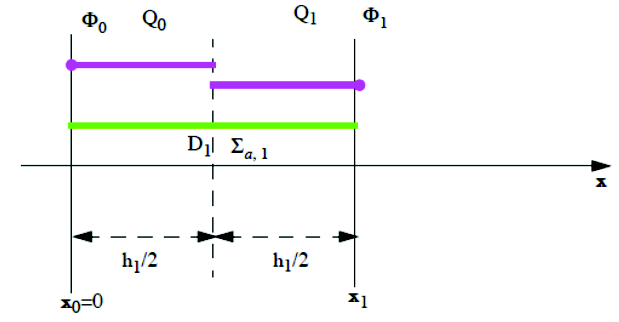
\includegraphics[height=2in]{ReflectingBC}
\end{figure}
%
\begin{align}
\int_{0}^{\frac{h_{1}}{2}} \biggl(-\frac{d}{dx}D(x)\frac{d \phi(x)}{dx}\biggr) dx &+ \int_{0}^{\frac{h_{1}}{2}} \Sigma_a(x) \phi(x) dx = \int_{0}^{\frac{h_{1}}{2}} S(x) dx \nonumber \\
%
-D(x)\frac{d \phi(x)}{dx}\big|_{\frac{h_{1}}{2}} &+ D(x)\frac{d \phi(x)}{dx}\big|_{0} + \Sigma_{a,1}\phi_0 \frac{h_1}{2} = S_0 \frac{h_1}{2} \nonumber 
\end{align}
%
Now we can apply the boundary condition $\frac{d \phi(x)}{dx}\big|_{0} = 0$ to get:
\[-D(x)\frac{d \phi(x)}{dx}\big|_{\frac{h_{1}}{2}} + \Sigma_{a,1}\phi_0 \frac{h_1}{2} = S_0 \frac{h_1}{2}\]

And the first equation ($i=0$) becomes
\[a_{00}^*\phi_0 + a_{01}^* \phi_1 = S_0\:,\]
%
where we redefine the $a$s to be (I've added the * to indicate that these have different definitions than the rest of the terms.)
%
\begin{align}
a_{00}^* &= \frac{2D_1}{h_1^2} + \Sigma_{a,1} \nonumber \\
a_{01}^* &= -\frac{2D_1}{h_1^2} \nonumber 
\end{align}

We now have $n$ equations and $n$ unknowns
\begin{equation}
\underbrace{\begin{pmatrix}
a_{00}^* & a_{01}^* & 0      & 0 & \cdots & 0 \\
a_{10}   & a_{11}   & a_{12} & 0 & \cdots & 0 \\
0        & a_{21}   & a_{22}   & a_{23} &  & \vdots \\
\vdots        &    & \ddots  & \ddots & \ddots & \vdots \\
0 & \cdots & 0 & a_{n-3,n-3}   & a_{n-2,n-2} & a_{n-2,n-1} \\
0        & \cdots   & 0   & 0 & a_{n-1,n-2} & a_{n-1,n-1} 
\end{pmatrix}}_{\ve{A}}
%
\underbrace{\begin{pmatrix}\phi_0 \\ \phi_1 \\ \phi_2 \\ \vdots \\ \phi_{n-2} \\ \phi_{n-1} \end{pmatrix}}_{\vec{\phi}} =
%
\underbrace{\begin{pmatrix}S_0 \\ S_1 \\ S_2 \\ \vdots \\ S_{n-2} \\ S_{n-1} \end{pmatrix}}_{\vec{S}}
\end{equation}

%----------------------------------------------------------------
\subsection{Homogeneous, Uniform Mesh}

If we end up having a homogeneous system with a uniform mesh, then we can make some simplifications.
%
\begin{align}
&h_i = h \nonumber \\
&D_i = D \nonumber \\
&\Sigma_{a,i} = \Sigma_a \nonumber \\
%
&\frac{-D}{h^2}\phi_{i-1} + \biggl(\frac{2D}{h^2} + \Sigma_a \biggr)\phi_i - \frac{D}{h^2}\phi_{i+1} = S_i \qquad \text{for } i = 1, \dots, n-2 \nonumber \\
%
&\biggl(\frac{2D}{h^2} + \Sigma_a \biggr) \phi_0 - \frac{D}{h^2}\phi_{1} = S_0 \qquad \text{for } i = 0 \nonumber \\
%
&\frac{-D}{h^2}\phi_{n-2} + \biggl(\frac{2D}{h^2} + \Sigma_a \biggr)\phi_{n-1} = S_{n-1} \qquad \text{for } i = n-1 \nonumber
\end{align}


%----------------------------------------------------------------
%----------------------------------------------------------------
\section{Solution Methods}

Both the FDM and FVM result in tridiagonal systems. Recall that formally solving these systems looks like
\[\vec{\phi} = \ve{A}^{-1}\vec{S} \:.\]
There are a few ways that we can solve these. 

%----------------------------------------------------------------
\subsection{Directly}

Tridiagonal systems can be solved directly using Gaussian elimination. 

This is not a bad option in our case because $\ve{A}$ is diagonally dominant (each diagonal element is greater than the sums of the absolute values of the off-diagonal elements in the same row):
\[a_{ii} \geq |a_{i,i-1}| + |a_{i, i+1}|\:.\] 

The general algorithm to solve a tridiagonal system is short and easy, it's called the \textbf{Thomas Algorithm}. We covered it back with general linear solution methods. 

%How do we develop an algorithm to execute this that can be easily programmed? 
\underline{Would you like to go through that a little more slowly or move to the next thing?}

Let's start by writing our system this way:
%
\begin{equation}
\begin{pmatrix}
B_0  & -C_0 & 0    & 0    & \cdots & 0 \\
-A_1 & B_1  & -C_1 & 0    & \cdots & 0 \\
0    & -A_2 & B_2  & -C_2 & & \vdots \\
\vdots        &    & \ddots  & \ddots & \ddots & \vdots \\
0 & \cdots & 0 & -A_{n-2} & B_{n-2} & -C_{n-2} \\
0        & \cdots   & 0   & 0 & -A_{n-1} & B_{n-1} 
\end{pmatrix}
%
\begin{pmatrix}\phi_0 \\ \phi_1 \\ \phi_2 \\ \vdots \\ \phi_{n-2} \\ \phi_{n-1} \end{pmatrix} =
%
\begin{pmatrix}S_0 \\ S_1 \\ S_2 \\ \vdots \\ S_{n-2} \\ S_{n-1} \end{pmatrix}
\end{equation}
%
Recall that $\phi_n = 0$. 

To develop the algorithm, let's look at a 3$\times$3 system of equations.
\begin{align}
B_0\phi_0 - C_0\phi_1 \hspace*{3.25em}&= S_0 \nonumber \\
-A_1\phi_0 + B_1\phi_1 - C_1\phi_2 &= S_1 \nonumber \\
-A_2\phi_1 + B_2\phi_2 &= S_2 \nonumber 
\end{align}
%
Now the process:
\begin{enumerate}
\item Define
\[u_0 = B_0 \qquad v_0 = S_0\]
and write the first equation as
\[u_0\phi_0 - C_0\phi_1 = v_0\]

\item multiply by $A_1 / u_0$
\[A_1\phi_0 - \frac{A_1 C_0}{u_0}\phi_1 = \frac{A_1 v_0}{u_0}\]
Now add this to the second equation (where the $\phi_0$ term subtracts out)
\[\biggl(B_1-\frac{A_1 C_0}{u_0}\biggr)\phi_1 - C_1\phi_2 = S_1 + \frac{A_1 v_0}{u_0}\]
%
and define
\[u_1 = B_1-\frac{A_1 C_0}{u_0} \qquad v_1 = S_1 + \frac{A_1 v_0}{u_0}\]
to re-write as
\[u_1\phi_1 - C_1\phi_2 = v_1\:.\]

\item Guess what's next? Multiply this equation by $A_2 / u_1$
\[A_2\phi_1 - \frac{A_2 C_1}{u_1}\phi_2 = \frac{A_2 v_1}{u_1}\]
and add to the third equation
\[\biggl(B_2-\frac{A_2 C_1}{u_1}\biggr)\phi_2 = S_2 + \frac{A_2 v_1}{u_1}\]
%
and define
\[u_2 = B_2-\frac{A_2 C_1}{u_1} \qquad v_2 = S_2 + \frac{A_2 v_1}{u_1}\]
to re-write as
\[u_2\phi_2 = v_2 \:.\]
\end{enumerate}
%
All together we now have an \textbf{upper triangular system}:
\begin{align}
u_0\phi_0 - C_0\phi_1 \hspace*{3.25em} &= v_0 \nonumber \\
u_1\phi_1 - C_1\phi_2 &= v_1 \nonumber \\
u_2\phi_2 &= v_2 \nonumber
\end{align}
%
that we can solve with \textbf{backward substitution}.

Here's the compact form of the algorithm (the Thomas algorithm)
\begin{enumerate}
\item \[u_0 = B_0 \qquad v_0 = S_0\]

\item for $i=1, \dots, n-1$
\[u_i = B_i-\frac{A_i C_{i-1}}{u_{i-1}} \qquad v_i = S_i + \frac{A_i v_{i-1}}{u_{i-1}}\]

\item Backward sub starting with $i=n-1$
\[\phi_{n-1} = \frac{v_{n-1}}{u_{n-1}}\]

\item Then for $i= n-2, \dots, 1$
\[\phi_i = \frac{1}{u_i}\bigl(v_i + C_i \phi_{i+1}\bigr)\]
\end{enumerate}

That was pretty easy,but we typically try to \textit{avoid direct inversion of matrices} because it might be expensive in time and/or memory, round-off error, instability, etc.

We often use an iterative method instead. 


%----------------------------------------------------------------
\subsection{Iterative Methods}

Recall: produce a sequence of vectors, $\vec{\phi}^{(1)}, \vec{\phi}^{(2)}, \dots$ based on the prescription
  \[\vec{\phi}^{(k+1)} = F(\vec{\phi}^{(k)}, \vec{S})\:, \qquad \text{where } \displaystyle \lim_{k \rightarrow \infty} \vec{\phi}^{(k)} = \vec{\phi}\] 
%
\begin{align}
(\ve{A} + \ve{B}) \vec{\phi} &= \ve{B}\vec{x} + \vec{S} \nonumber \\
%
\ve{C} \vec{\phi} &= \ve{B}\vec{\phi} + \vec{S} 
\qquad\text{where } \ve{C} = \ve{A} + \ve{B} \nonumber \\
%
\vec{\phi} &= \ve{C}^{-1} \ve{B}\vec{\phi} + \ve{C}^{-1} \vec{S} 
\nonumber \\
%
\vec{\phi} &= \ve{P}\vec{\phi} + \tilde{\vec{S}}  
\qquad\text{assuming regular } \ve{C}\nonumber
\end{align}
%
And the \textbf{fixed-point} iterative process is:
\begin{align}
\vec{\phi}^{(0)} &= \text{ arbitrary}\nonumber \\
\vec{\phi}^{(k+1)} &= \ve{P}\vec{\phi}^{(k)} + \tilde{\vec{S}} \nonumber
\end{align}

How we split $\ve{A}$ determines what method we're doing.

\subsubsection{Jacobi}

Let $\ve{D} = diag(\ve{A})$, then
\begin{align}
\ve{D} \vec{\phi}^{k+1} &= (\ve{D} - \ve{A})\vec{\phi}^{(k)} + \vec{S} \nonumber \\
%
\vec{\phi}^{k+1} &= \ve{D}^{-1}(\ve{D} - \ve{A})\vec{\phi}^{(k)} + \ve{D}^{-1}\vec{S} \nonumber
\end{align}
%
In our original syntax, $\ve{P}_J = \ve{I} -  \ve{D}^{-1}\ve{A}$ and $\tilde{\vec{S}} =\ve{D}^{-1}\vec{S}$.

The algorithm for this method is, for $i = 1, \dots, n$:
\[ \phi^{(k+1)}_i = \frac{1}{a_{ii}}(S_i - \sum_{j=1}^{i-1} a_{ij} \phi_j^{(k)} - \sum_{j=i+1}^{n} a_{ij} \phi_j^{(k)})\]

We can apply Gauss Seidel and SOR in exactly the same way. 




%--------------------------------------------------------------------
%--------------------------------------------------------------------
%\bibliographystyle{plain}
%\bibliography{LinearSolns} 

\end{document}